\documentclass{beamer}
\usepackage[utf8]{inputenc} % allow utf-8 input
\usepackage[T1]{fontenc}    % use 8-bit T1 fonts
\usepackage{hyperref}       % hyperlinks
\usepackage{url}            % simple URL typesetting
\usepackage{booktabs}       % professional-quality tables
\usepackage{amsfonts}       % blackboard math symbols
\usepackage{nicefrac}       % compact symbols for 1/2, etc.
\usepackage{microtype}      % microtypography
\usepackage{amsmath}
\usepackage{mathtools}
\usepackage{tikz}
\usetikzlibrary{calc}
\usetikzlibrary{bayesnet}
\usetikzlibrary{arrows}
\usepackage{color}
\usepackage{array}
\usepackage{dsfont}
\usepackage{multirow, graphicx}
 \usepackage{float}
\newcolumntype{C}[1]{>{\centering\arraybackslash}p{#1}}
\newcolumntype{R}[1]{>{\raggedleft\arraybackslash}p{#1}}
\newcolumntype{L}[1]{>{\raggedright\arraybackslash}p{#1}}
\usepackage{caption}
\usepackage{subfig}
\usepackage{pifont}
\usepackage{xcolor}
\usepackage{algorithm,algorithmic}
% \floatname{algorithm}{Procedure}
\renewcommand{\algorithmicrequire}{\textbf{Input:}}
\renewcommand{\algorithmicensure}{\textbf{Output:}}
\newcommand{\cmark}{\textcolor{green!80!black}{\ding{51}}}
\newcommand{\xmark}{\textcolor{red}{\ding{55}}}
\DeclareMathOperator*{\argmin}{argmin}
\urlstyle{same}
\usepackage{listings}
\usepackage[export]{adjustbox}
\usepackage{inconsolata}
% \usetheme{Boadilla}

\title{Attention is All You Need}
% \subtitle{Using Beamer}
\author{Bill Watson}
\institute{S\&P Global}
\date{November 22, 2019}

\newenvironment{nospaceflalign*}
 {\setlength{\abovedisplayskip}{0pt}\setlength{\belowdisplayskip}{0pt}%
  \csname flalign*\endcsname}
 {\csname endflalign*\endcsname\ignorespacesafterend}

\AtBeginSection[]{
  \begin{frame}
  \vfill
  \centering
  \begin{beamercolorbox}[sep=8pt,center,shadow=true,rounded=true]{title}
    \usebeamerfont{title}\insertsectionhead\par%
  \end{beamercolorbox}
  \vfill
  \end{frame}
}

\begin{document}

\begin{frame}
\titlepage
\end{frame}


\begin{frame}
\frametitle{Recap: Encoder-Decoder Models}

\end{frame}

\begin{frame}
\frametitle{How can we improve this model?}
\begin{itemize}
  \item Add an alignment model to force the model to 'attend' to different parts of the input
  \item Gives model acess to the encodings for the input directly
\end{itemize}
\end{frame}

\begin{frame}
\frametitle{What are Context Vectors?}
\begin{equation*}
  c_i = \sum_{j} \alpha_{ij} \cdot h_j
\end{equation*}
\begin{itemize}
  \item A \textbf{context vector} $c_i$ is the weighted sum of the encodings for the $i$-th iteration of the decoder
  \item $s_{i-1}$ is the previous hidden state of the decoder
  \item $h_j$ is the encoding for the $j$-th input word
  \item $\alpha_ij$ is the weight associated for the $j$-th input word for the $i$-th deocding iteration
\end{itemize}
\end{frame}

%%%%%%%%%%%%%%%%%%%%%%%%%%%%%%%%%%%%%%%%%%%%%%%%%%%%%%%%%%%%%%%%%%%%%%%%%%%%%%%%
\section{(Simple) Attention Mechanisms}

\begin{frame}
\frametitle{Mean Attention}
\begin{equation*}
  \begin{split}
  \alpha_ij &= \frac{1}{J} \\
  c_i &= \frac{1}{J} \sum_j^J h_j = \sum_{j} \alpha_{ij} \cdot h_j
  \end{split}
\end{equation*}
\begin{itemize}
  \item Very simple and naive approach is to apply uniform weights to each encoding $h_j$
  \item Fancy way of saying average
  \item $J$ is the length of the source sentence
\end{itemize}
\end{frame}

\begin{frame}
\frametitle{Location Based: Laplace}
\begin{equation*}
  \begin{split}
  \alpha_{ij} &= f \left(j \mid i, b \right) = \frac{1}{2b} \exp \left( - \frac{\lvert j - i \rvert}{b} \right) \\
  c_i &= \sum_{j} \alpha_{ij} \cdot h_j
  \end{split}
\end{equation*}
\begin{itemize}
  \item Weighted by location in sequence
  \begin{itemize}
    \item Center a Laplace at $\mu=i$, scale $b$
    \item Weight is the probability of position $j$ relative to $i$
  \end{itemize}
  \item Penalizes elements away from the diagonal
  \item Heavier tail than a Gaussian
\end{itemize}
\end{frame}

\begin{frame}
\frametitle{Location Based: Gaussian}
\begin{equation*}
  \begin{split}
  \alpha_{ij} &= f \left(j \mid i, \sigma^2 \right) = \frac{1}{\sqrt{2\pi\sigma^2}} \exp \left( - \frac{\left( j - i \right)^2}{2\sigma^2} \right) \\
  c_i &= \sum_{j} \alpha_{ij} \cdot h_j
  \end{split}
\end{equation*}
\begin{itemize}
  \item Weighted by location in sequence
  \begin{itemize}
    \item Center a Gaussian at $\mu=i$, scale $\sigma$
    \item Weight is the probability of position $j$ relative to $i$
  \end{itemize}
  \item Smoother distribution closer to the diagonal
  \item Smaller tail than Laplace, so outliers are penalized more
\end{itemize}
\end{frame}

\begin{frame}
\frametitle{Visualizing Location-Based Distributions}
\begin{columns}
  \begin{column}{0.45\textwidth}
    \begin{figure}
      \centering
      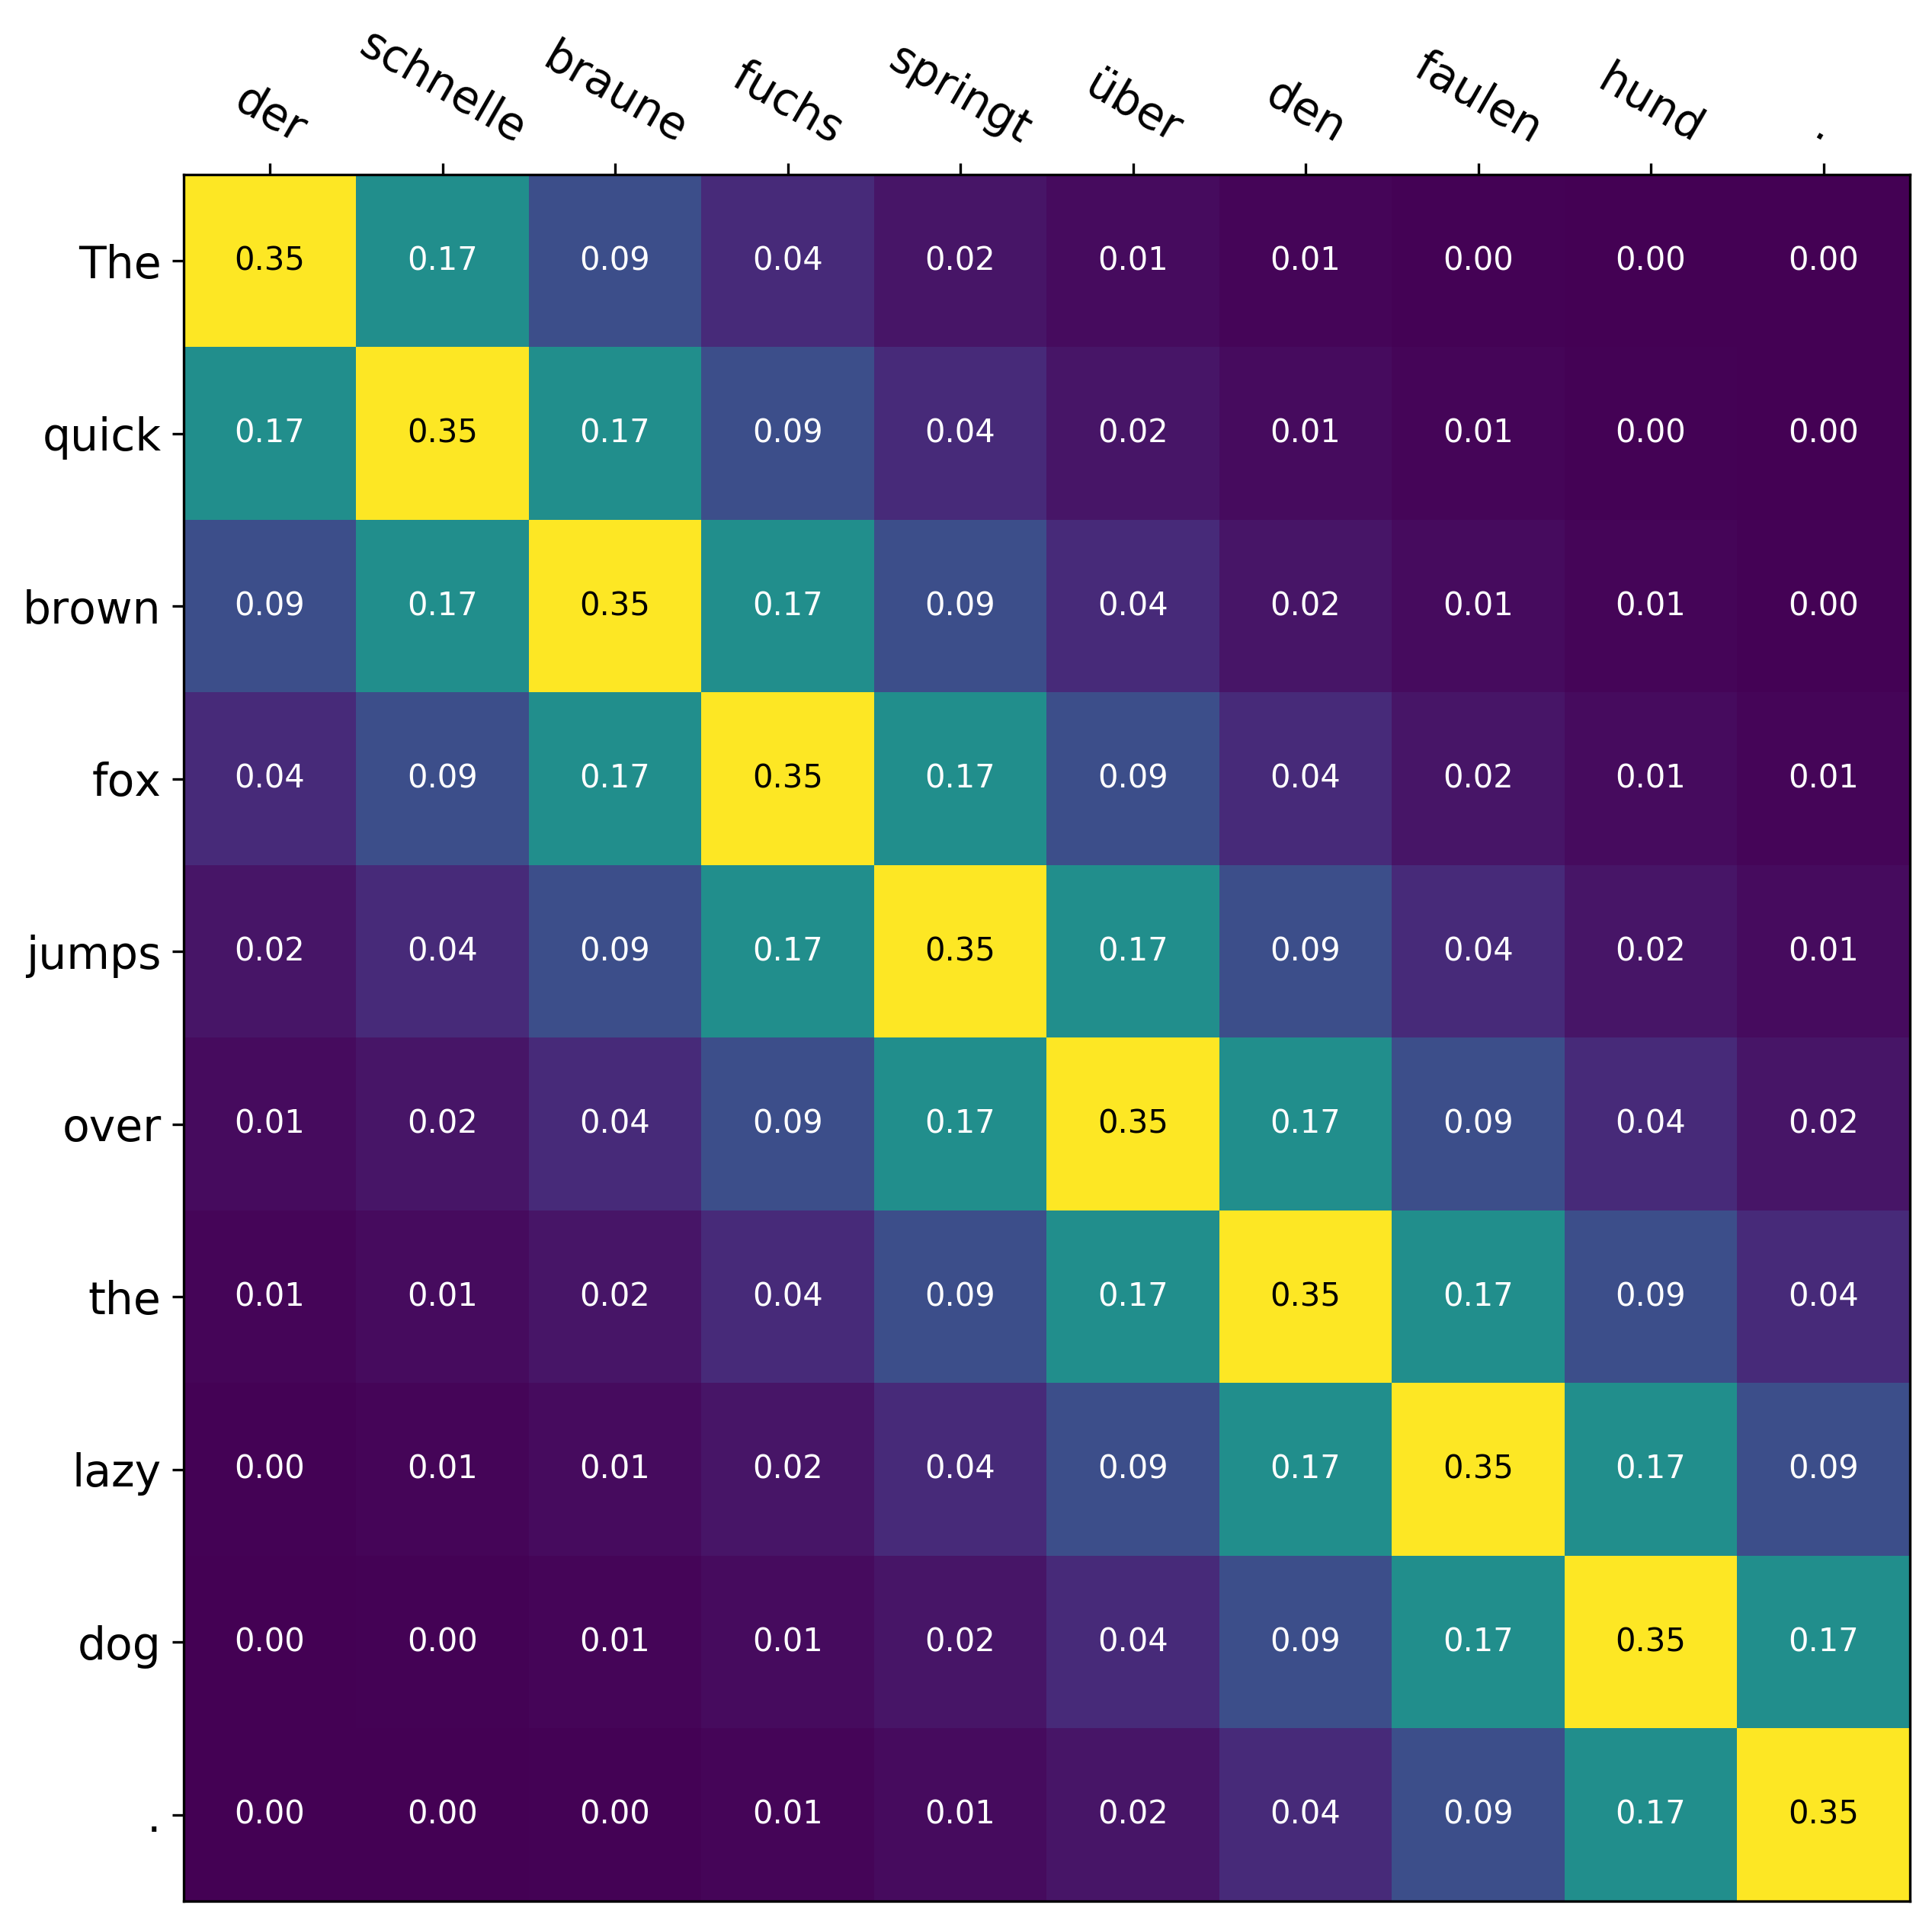
\includegraphics[width=4.75cm, valign=c]{assets/laplace}
      \caption{Laplace}
    \end{figure}
  \end{column}
  \begin{column}{0.45\textwidth}
    \begin{figure}
      \centering
      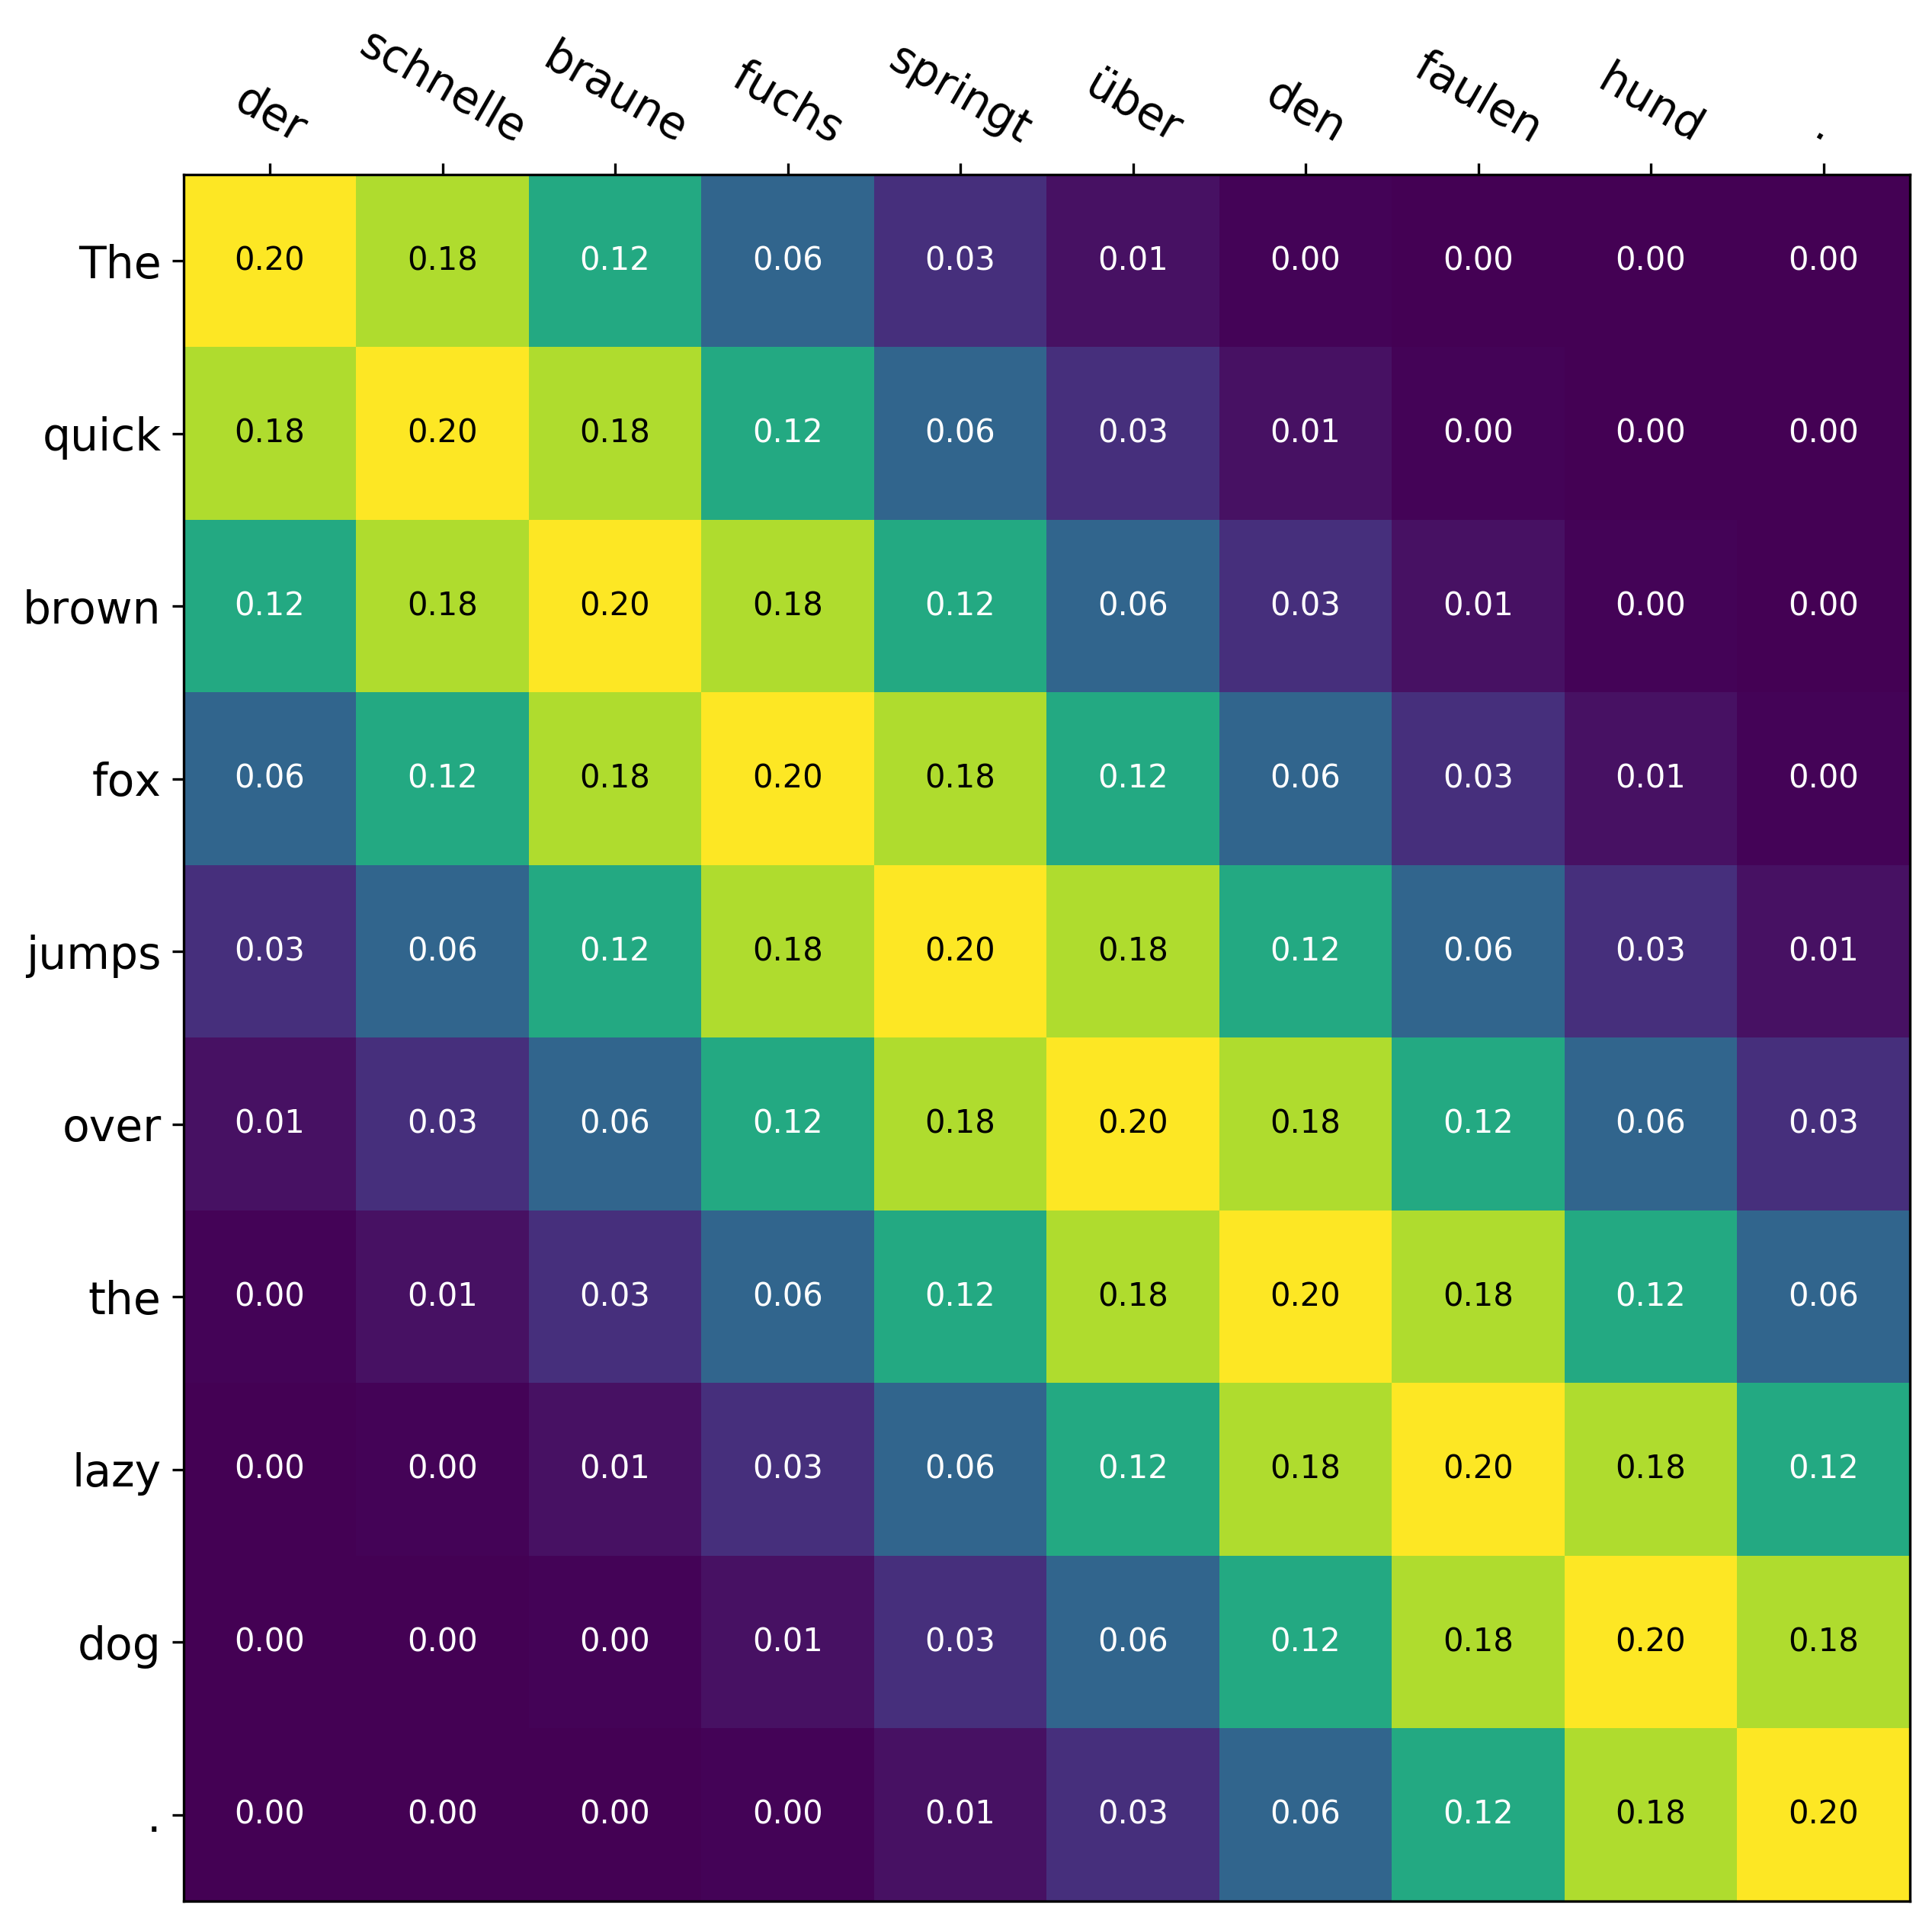
\includegraphics[width=4.75cm, valign=c]{assets/normal}
      \caption{Gaussian}
    \end{figure}
  \end{column}

\end{columns}
\end{frame}


%%%%%%%%%%%%%%%%%%%%%%%%%%%%%%%%%%%%%%%%%%%%%%%%%%%%%%%%%%%%%%%%%%%%%%%%%%%%%%%%
\section{(Parameter-based) Attention Mechanisms}

\begin{frame}
\frametitle{Parameter-based Attention}
% rework
\begin{itemize}
  \item Why not use learnable weights to effectively mix the encodings?
  \item Let deep learning figure out the alignment
  \item We know define a scoring function conditioned on the previous hidden state and input encoding
\end{itemize}
\begin{equation*}
  a\left( s_{i-1}, h_j \right) = ?
\end{equation*}
\begin{itemize}
  \item In order to constrain the weights to a valid distribution, we softmax
\end{itemize}
\begin{equation*}
  \begin{split}
    \alpha_{ij} &= \frac{\exp\left( a\left( s_{i-1}, h_j \right) \right)}{\sum_k \exp\left( a\left( s_{i-1}, h_k \right) \right)}\\
    c_i &= \sum_{j} \alpha_{ij} \cdot h_j
  \end{split}
\end{equation*}
\end{frame}

\begin{frame}
\frametitle{Bahdanau Attention}
\begin{equation*}
  a\left( s_{i-1}, h_j \right) = v_a^T \tanh \left( W_a s_{i-1} + U_a h_j + b \right)
\end{equation*}
\end{frame}


\begin{frame}
\frametitle{Luong Attention: Dot Product}
\begin{equation*}
  a\left( s_{i-1}, h_j \right) = s_{i-1}^T h_j
\end{equation*}
\end{frame}

\begin{frame}
\frametitle{Luong Attention: Scaled Dot Product}
\begin{equation*}
  a\left( s_{i-1}, h_j \right) = \frac{1}{\sqrt{\lvert h_j \rvert}} s_{i-1}^T h_j
\end{equation*}
\end{frame}

\begin{frame}
\frametitle{Luong Attention: General}
\begin{equation*}
  a\left( s_{i-1}, h_j \right) = s_{i-1}^T W_a h_j
\end{equation*}
\end{frame}

\begin{frame}
\frametitle{Luong Attention: Local Attention}
\begin{equation*}
  a\left( s_{i-1}, h_j \right) = W_a s_{i-1}
\end{equation*}
\end{frame}

%%%%%%%%%%%%%%%%%%%%%%%%%%%%%%%%%%%%%%%%%%%%%%%%%%%%%%%%%%%%%%%%%%%%%%%%%%%%%%%%
\section{(Advanced) Attention Mechanisms}

\begin{frame}
\frametitle{Fine-Grained Attention}
\begin{equation*}
  a^k \left( s_{i-1}, h_j \right) = \texttt{FF}^k(s_{i-1}, h_j)
\end{equation*}
\begin{equation*}
  \alpha_{ij}^d = \frac{\exp\left(a^d\left(s_{i-1}, h_j\right)\right)}{\sum_k \exp \left( a^d \left(s_{i-1}, h_k\right) \right)}
\end{equation*}
\begin{equation*}
  c_i = \sum_j \alpha_{ij} \odot h_j
\end{equation*}
\end{frame}

\begin{frame}
\frametitle{Multi-Headed Attention}
\begin{equation*}
  \alpha_{ij}^d = \frac{\exp\left(a^d\left(s_{i-1}, h_j\right)\right)}{\sum_k \exp \left( a^d \left(s_{i-1}, h_k\right) \right)}
\end{equation*}

\begin{equation*}
  \alpha_{ij} = \frac{1}{k} \sum_k \alpha^k_{ij}
\end{equation*}
\end{frame}

\begin{frame}
\frametitle{Self Attention}
\begin{equation*}
  a_{ij} = \frac{1}{|h|} h_{j}h_k^T
\end{equation*}

\begin{equation*}
  \alpha_{jk} = \frac{\exp\left( a_{jk} \right)}{\sum_k \exp \left( a_{jk} \right)}
\end{equation*}

\begin{equation*}
  \texttt{self-attention}\left( h_j \right) = \sum_k \alpha_{jk} h_k
\end{equation*}
\end{frame}

\section{Practical Considerations}

\begin{frame}
\frametitle{Masking}

\end{frame}

\begin{frame}
\frametitle{Which one to use?}

\end{frame}

\begin{frame}
\frametitle{Mixing and Matching}

\end{frame}

%%%%%%%%%%%%%%%%%%%%%%%%%%%%%%%%%%%%%%%%%%%%%%%%%%%%%%%%%%%%%%%%%%%%%%%%%%%%%%%%

\section{Tools, References, and Further Reading}


\begin{frame}
\frametitle{Papers}
  \begin{itemize}
    \item \href{https://arxiv.org/pdf/1409.0473}{Bahdanau et al., Neural Machine Translation by Jointly Learning to Align and Translate}
    \item \href{https://arxiv.org/pdf/1508.04025}{Luong et al.m Effective Approaches to Attention-based Neural Machine Translation}
    \item \href{https://papers.nips.cc/paper/7181-attention-is-all-you-need.pdf}{Vaswani et al., Attention is All You Need}
    \item \href{http://www.aclweb.org/anthology/N13-1073}{Dyer et al., A Simple, Fast, and Effective Reparameterization of IBM Model 2}
  \end{itemize}
\end{frame}


% Refs, ideas, etc


\end{document}
